\subsubsection{Package Util}

The Util subsystem contains the Verbose class, which handles the models logging. Any logs generated by the model are sent to the Verbose class, which is a subject in the Observer design pattern. The Verbose class is a singleton, and when the Verbose objects log() method is called, it alerts any of its Observers to a change in its state, and allows them to retrieve the message being logged, in accordance with the Observer pattern.

\paragraph{Detailed Design Diagram}\mbox{}
\begin{figure}[H]
\centering
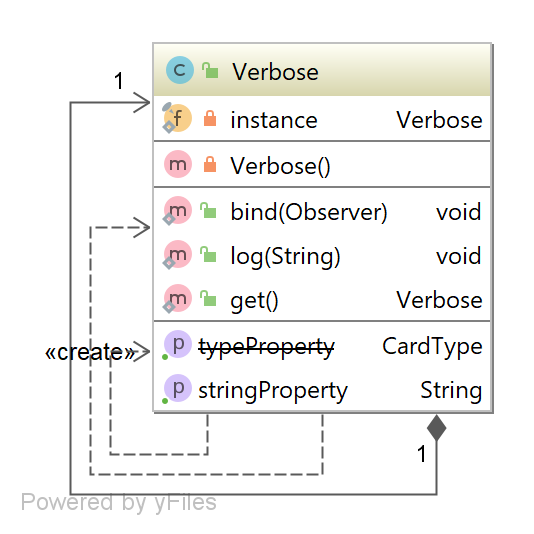
\includegraphics[width=10cm]{Source/Module/Model/Util/Model_Util.png}
\caption{UML Diagram of Package Util in Module Model}
\label{Model.Util}
\end{figure}

\paragraph{Class Verbose}\mbox{}
\begin{tabularx}{\textwidth}{|c||l|l|l|X|}
    \hline
    \cellcolor{lightgray}Class Name & \multicolumn{4}{X|}{Verbose}\\
    \hline
    \cellcolor{lightgray}Inherits From & \multicolumn{4}{X|}{extends Subject}\\
    \hline
    \cellcolor{lightgray}Description & \multicolumn{4}{p{12cm}|}{Part of the Observer pattern. The model's interface to the view's VerboseView, used to log things which are optionally printed to a GUI.}\\

    \hline\hline
    \cellcolor{lightgray}Attributes & \cellcolor{lightgray}Visibility & \cellcolor{lightgray}Data type & \cellcolor{lightgray}Name & \cellcolor{lightgray}Description\\\cline{2-5}
    \cellcolor{lightgray} & Private & Verbose & instance & The verbose instance to which observers can be attached.\\\cline{2-5}
    \cellcolor{lightgray} & Private & String & state & The message currently being displayed.\\ 
    \hline\hline
    \cellcolor{lightgray}Methods & \cellcolor{lightgray}Visibility & \multicolumn{2}{l|}{\cellcolor{lightgray}Method Name} & \cellcolor{lightgray}Description\\\cline{2-5}
    \hline
    \cellcolor{lightgray} & Private & \multicolumn{2}{l|}{Verbose()} & Constructor.\\
    \hline
    \cellcolor{lightgray} & Public & \multicolumn{2}{l|}{bind(Observer o)} & Attaches the observer to the instance so it will be alerted if the state changes. \\
    \hline
    \cellcolor{lightgray} & Public & \multicolumn{2}{l|}{log(String arg)} & Sets the state to a new message and alerts observers. \\
    \hline
    \cellcolor{lightgray} & Public & \multicolumn{2}{l|}{get()} & Returns the instance.\\
    \hline
    \cellcolor{lightgray} & Public & \multicolumn{2}{l|}{getStringProperty()} & Returns the current message.\\
    \hline
    \cellcolor{lightgray} & Public & \multicolumn{2}{l|}{getTypeProperty()} & Returns nothing, deprecated.\\
    \hline
\end{tabularx}